\documentclass[dvipdfmx]{jsarticle}

\title{西暦和暦変換プログラムの作成(Java版)}
\author{Seiichi Nukayama}
\date{2020-05-05}
\usepackage{tcolorbox}
\usepackage{color}
\usepackage{listings, plistings}

% Java
\lstset{% 
  frame=single,
  backgroundcolor={\color[gray]{.9}},
  stringstyle={\ttfamily \color[rgb]{0,0,1}},
  commentstyle={\itshape \color[cmyk]{1,0,1,0}},
  identifierstyle={\ttfamily}, 
  keywordstyle={\ttfamily \color[cmyk]{0,1,0,0}},
  basicstyle={\ttfamily},
  breaklines=true,
  xleftmargin=0zw,
  xrightmargin=0zw,
  framerule=.2pt,
  columns=[l]{fullflexible},
  numbers=left,
  stepnumber=1,
  numberstyle={\scriptsize},
  numbersep=1em,
  language={Java},
  lineskip=-0.5zw,
  morecomment={[s][{\color[cmyk]{1,0,0,0}}]{/**}{*/}},
}
%\usepackage[dvipdfmx]{graphicx}
\usepackage{url}
\usepackage[dvipdfmx]{hyperref}
\usepackage{amsmath, amssymb}
\usepackage{itembkbx}
\usepackage{eclbkbox}	% required for `\breakbox' (yatex added)
\fboxrule=1pt
\parindent=1em
\begin{document}

\pagenumbering{arabic}

%% 修正時刻: Wed May  6 07:18:47 2020


\section{}
\pagenumbering{arabic}

\subsection{{\Large 課題5}}

\begin{breakbox}
 前回までで作成した Nengo.java Xnengo.java を Servlet \& JSP にします。
 パッケージ名は、com.example.nengo。
 JSPのファイル名は任意ですが、index.jsp が簡単でいいかもしれません。
\end{breakbox}

\subsection{\large ヒント1}

\subsubsection{入力画面}

ユーザーが入力する画面をつくります。

ユーザーには二つの選択肢があります。

一つは、西暦を入力して、年号と年を求めるという選択。

もう一つは、年号と年を入力して、その西暦年を求めるという選択。

いずれかを選択してボタンをクリックすると、答えが表示されるようにします。

これは、入力画面の例です。

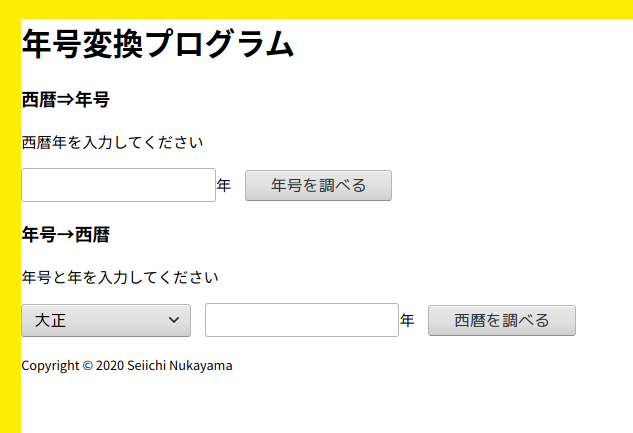
\includegraphics[width=10cm]{gamen01.png}

\subsubsection{処理の流れ}

おおまかに、どういう処理の流れにするかを考えます。

これは一つの例です。
ファイル名も例です。

\textgt{選択肢1}
\begin{enumerate}
 \item 入力画面で西暦を入力 \textgt{index.jsp}
 \item 西暦から年号と年を調べるサーブレットで受け取る \textgt{Xnengo.java}
 \item (サーブレットの中の処理) Nengo.class を使って、年号を求める \textgt{Nengo.java}
 \item 求めた年号と年を入力画面に返す。 \textgt{Xnengo.java}
 \item 入力画面で表示 \textgt{index.jsp}
\end{enumerate}

\textgt{選択肢2}
\begin{enumerate}
 \item 入力画面で年号と年を入力 \textgt{index.jsp}
 \item 年号と年から西暦を調べるサーブレットで受け取る \textgt{Xseireki.java}
 \item (サーブレットの中の処理) Nengo.class を使って、西暦を求める \textgt{Nengo.java}
 \item 求めた西暦を入力画面に返す。 \textgt{Xseireki.java}
 \item 入力画面で表示 \textgt{index.jsp}
\end{enumerate}

\subsubsection{データの受け渡しの方法}

最初の入力画面(index.jsp)からサーブレット(Xnengo.java, Xseireki.java)へのデータの受け渡しは、\textgt{POST} を使うことにします。( GET でもいんですが、とりあえず)

サーブレット内で、西暦から年号への変換、年号から西暦への変換は、今までに作成した Nengo.java をそのまま使うことにします。\textgt{toNengo}メソッド、\textgt{toSeireki}メソッドがそのまま使えます。

サーブレットから入力画面(index.jsp)へのデータの受け渡しには、セッション変数を使うことにします。

サーブレット内で以下のような式を記述するだけでセッション変数を使えます。

\verb!HttpSession session = request.getSession(true);!

このように 変数session を宣言して、次のように使います。

\verb!session.setAttribute("nengo", nengo);!

これは、"nengo"というセッション変数に nengo という値をセットしています。

そして、これを入力画面(index.jsp)で、以下のように取り出します。

\begin{verbatim}
<%
nengo = session.getAttribute("nengo");
%>
\end{verbatim}

そして、これを \verb!<html><body>~</body><html>! の \verb!<body>!の中で、
\verb!<%= nengo %>! とすることで、画面に表示できます。


%%=====================================================================
\section{\Large 解答例}

\subsection{{\Large 手順}}

\subsubsection{\large Eclipseで新規プロジェクトを作成}

''ファイル'' - ''新規'' - ''動的Webプロジェクト''

''プロジェクト名''は「nengo」

「次へ」-「次へ」とクリックし、''Web.xmlデプロイ記述子の作成''にチェック
を入れる。(もしチェックし忘れても、あとで作れるから大丈夫)


\subsubsection{\large JSPファイルを作成}

''nengo''を右クリックして、''新規'' - ''JSPファイル''

''親フォルダー'' は ''nengo/WebContent'' のままでよい。

''ファイル名'' に、「index.jsp」と入力。

''次へ'' で、''JSPテンプレートの選択'' となるから、
「新規JSPファイル(HTML5)」を選択。そして ''完了''。

index.jsp は以下のようにする。

\begin{lstlisting} [caption=index.jsp]
<%@ page language="java" contentType="text/html; charset=UTF-8"
         pageEncoding="UTF-8" %>
<!doctype html>
<html lang="ja">
  <head>
    <meta charset="utf-8"/>
    <title>年号変換プログラム</title>
    <link rel="stylesheet" href="css/nengo.css"/>
  </head>
  <body>
    <div id="wrap">
      <header>
        <h1>年号変換プログラム</h1>
      </header>
      <article>
        <section>
          <h1>西暦⇒年号</h1>
          <form action="/nengo/Xnengo" method="post">
            <p>西暦年を入力してください</p>
            <p><input type="text" name="seireki" id="seireki"/>年
              &nbsp;&nbsp;
              <input type="submit" value="年号を調べる"/></p>
          </form>
          <div id="kaito-nengo"></div>
        </section>
        <section>
          <h1>年号⇒年西暦</h1>
          <form action="/nengo/Xseireki" method="post">
            <p>年号と年を入力してください</p>
            <p><select name="nengo" id="nengo">
              <option value="" selected>選択してください</option>
              <option value="meiji">明治</option>
              <option value="taisyo">大正</option>
              <option value="syouwa">昭和</option>
              <option value="heisei">平成</option>
              <option value="reiwa">令和</option>
              <option value="mirai">未来</option>
            </select>
            &nbsp;&nbsp;
            <input type="text" name="nen" id="nen"/>年
            &nbsp;&nbsp;
            <input type="submit" value="西暦を調べる"/></p>
          </form>
          <div id="kaito-seireki"></div>
        </section>
      </article>
      <footer>
        <small>Copyright &copy; 2020 Seiichi Nukayama</small>
      </footer>
    </div>
  </body>
</html>
\end{lstlisting}

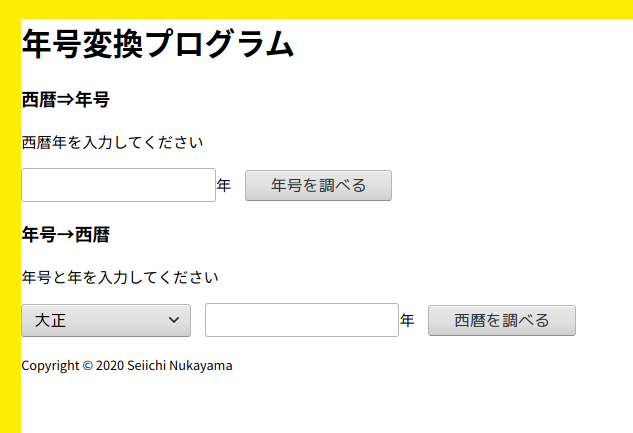
\includegraphics[width=10cm]{gamen01.png}

このコードの特徴は、西暦から年号を求めるフォームと、年号から西暦を求めるフォームの2種類があることで、西暦から年号を求めるフォームは ''Xnengo''サーブレットに処理を渡しています。年号から西暦を求めるフォームは ''Xseireki''サーブレットに処理を渡しています。


\subsubsection{\large サーブレットを作成}

まず、''Xnengo''サーブレットを作成します。
これは、index.jspの ''年号を求める''ボタンを押すと、このサーブレットにデータが送られます。

プロジェクトの ''nengo'' を右クリックして、''新規'' - ''サーブレット'' を選択します。''サーブレット作成''ダイアログが開くので、以下のように入力します。

''ソース・フォルダー'' は、そのまま(/nengo/src)。

''Javaパッケージ'' は、「com.example.nengo」とします。

''クラス名''は、「Xnengo」とします。

''スーパークラス''は、そのままでいいです。(javax.servlet.http.HttpServlet)

「完了」をクリックすると、Xnengoサーブレットのひな型でひらきます。

今回は、POSTしか使いませんので、''doGet''メソッドは削除してください。

また、''doPost''メソッドの中の ''doGet(request, response)'' は、削除して
おいてください。

そして、''doPost''メソッドを以下のようにしてください。

\begin{verbatim} [caption=Xnengo.java]
protected void doPost(HttpServletRequest request, HttpServletResponse
        response) throws ServletException, IOException {

    // JSPから受け取る文字列を UTF-8 とします。
    request.setCharacterEncoding("UTF-8");

    // index.jspにデータを送り返すのに、セッションという
    // しくみを使います。
    HttpSession session = request.getSession(true);    // --- <1>

    // index.jspから送られてきたデータ(seireki)を
    // 受け取って、txtSeirekiという文字列にセット。
    String txtSeireki = request.getParameter("seireki"); // --- <2>

    // index.jspからのデータが null あるいは 空 の場合
    if (txtSeireki != null && txtSeireki != "") {      
        this.toNengo(txtSeireki);                      // --- <3>
        session.setAttribute("nengo", this.nengo);     // --- <4>
        session.setAttribute("nen", this.nen)
        session.setAttribute("error", null);
        session.setAttribute("seireki", null);
    }
    else {
        session.setAttribute("nengo", null);           // --- <5>
        session.setAttribute("nen", null);
        session.setAttribute("seireki", null);
        session.setAttribute("error", this.ERROR);
    }
    response.sendRedirect("/nengo");                   // --- <6>
}
\end{verbatim}

\begin{enumerate}
 \item \textgt{セッション変数}を使ってクライアント(index.jspをダウンロー
       ドしたユーザーのブラウザ)にデータを送ります。
 \item \textgt{post}で送られてきた \textgt{seireki} というラベルがつけら
       れたデータを取得。
 \item \textgt{Xnengo}クラスのメソッド \textgt{toNengo}に seirekiデータ
       を送り、クラス変数 this.nengo と this.nen に年号と年をセットしま
       す。このメソッドは後ほど作ります。
 \item セッション変数''nengo''に、this.nengo をセットします。このセッショ
       ン変数は、クライアントのブラウザに送られます。
 \item クライアントから post で seireki データが送られてこなかった場合、
       クライアントのブラウザに送るセッション変数には ``null''をセットし
       ます。これは、``''でもいいかもしれません。
 \item http://XXXXXXX/nengo というURLにアクセスするようにクライアントに
       指示します。       
\end{enumerate}






Eclipseを起動して、新規プロジェクトを作成します。

パッケージ名を''com.example.nengo''とします。



ディレクトリを以下のようにする。

\begin{tcolorbox}
 /home/\$HOME/work/Lala/jsp/nengo
\end{tcolorbox}

これをTomcatに登録する。

\verb!$CATALINA_HOME/conf/Catalina/localhost! に以下のファイルをおく。

\begin{lstlisting}[caption=nengo.xml]
 <?xml version="1.0" encoding="utf-8" ?>
 <Context path="/nengo" docBase="/home/(ユーザー名)/work/Lala/jsp/nengo" />
\end{lstlisting}

\verb!/home/$HOME/work/Lala/jsp/nengo! を以下のように構成する。

\begin{verbatim}
./
├── WEB-INF
│   ├── classes
│   ├── lib
│   └── web.xml
├── css
│   └── nengo.css
├── index.jsp
└── src
     └── com
         └── example
             └── nengo
                 ├── Nengo.java
                 └── Xnengo.java
\end{verbatim}

\subsubsection{{\large 初期ファイル}}

web.xml は以下のようにする。

\begin{lstlisting} [caption=web.xml]
 <?xml version="1.0" encoding="UTF-8" ?>
<web-app>
    <servlet>
        <servlet-name>nengo</servlet-name>
        <servlet-class>com.example.nengo.Nengo</servlet-class>
    </servlet>
    <servlet-mapping>
        <servlet-name>nengo</servlet-name>
        <url-pattern>/nengo</url-pattern>
    </servlet-mapping>
</web-app>
\end{lstlisting}

さて、index.jsp からポストされたデータは、com.example.nengo.Xnengo サー
ブレットで受け取る。

 \begin{lstlisting} [caption=WEB-INF/src/com/example/nengo/Xnengo.java]
// Xnengo.java
package com.example.nengo;

import javax.servlet.*;
import javax.servlet.http.*;
import java.io.*;
import java.util.*;

public class Xnengo extends HttpServlet {
    private static final long serialVersionUID = 1L;

    private int seireki = 0;
    private String nengo = "";
    private int nen = 0;
    private final String ERROR = "エラーです";
    
    
    protected void doPost( HttpServletRequest request, HttpServletResponse response )
        throws ServletException, IOException {
        request.setCharacterEncoding("UTF-8");

        HttpSession session = request.getSession(true);
        
        String txtSeireki = request.getParameter("seireki");
        if (txtSeireki != null && txtSeireki != "") {
            this.toNengo(txtSeireki);
            session.setAttribute("nengo", this.nengo);
            session.setAttribute("nen", this.nen);
            session.setAttribute("error", null);
        } else {
            session.setAttribute("nengo", null);
            session.setAttribute("nen", null);
            session.setAttribute("error", this.ERROR);
        }
        response.sendRedirect("/nengo");
    }

    private void toNengo(String txtSeireki) {
        int s = Integer.parseInt(txtSeireki);
        Nengo n = new Nengo();
        n.toNengo(s);
        this.nengo = n.getNengo();
        this.nen = n.getNen();
    }
} 
 \end{lstlisting}




 
\end{document}

%% 修正時刻: Sat May  2 15:10:04 2020


%% 修正時刻: Sat May  9 12:45:37 2020
